\section{Implementation} \label{sec:implementation}
% Tobias

% Forward / Backward engineering
When creating the database we used forward engineering to auto generate the 
database from a MySQL EER diagram. The diagram can be seen in 
Figure~\ref{fig:EER}. This had the advantage that the EER diagram could easily 
be made as a translation of the ER Diagram described in 
Section~\ref{sec:design}. This means that it was relatively easy to 
implementation the database, in accordance with the design. We only had to make 
sure that our translation from the ER diagram to the MySQL EER diagram was 
correct to guarantee that the implemented database worked as desired. However, 
this proved more difficult than expected. Because although it could be directly 
translated, it did happen that the way we actually wanted to implement it, was 
not strictly in accordance with the translation of the design. This sometimes 
resulted in changes of the design, as we realized the design was not in 
accordance with the desired functionality. Other times the desired effect was 
achieved although not in accordance with the translation. This can be seen in 
the weak relations \emph{from} and \emph{to} in which the entity \emph{Track} 
has total participation. In order to ensure the total participation, 
\emph{from} and \emph{to} could be primary keys in the entity \emph{Track}. But 
since we wanted to allow having multiple parallel tracks, we made the attribute 
\emph{Id} the primary key. Obviously, we could have made a combined primary 
key, from all three attributes, but this would have allowed for duplicate Ids, 
which we were not interested in. We therefore kept the Id as the primary key, 
and ensured the existence of \emph{from} and \emph{to} by disallowing them from 
being \emph{null}.

\subsection{MySQL EER Diagram}

As described above the EER diagram, seen in Figure~\ref{fig:EER}, was made from 
the hand drawn Entity Relation Diagram show in Figure~\ref{fig:ER}.

\begin{figure}[h]
    \centering
    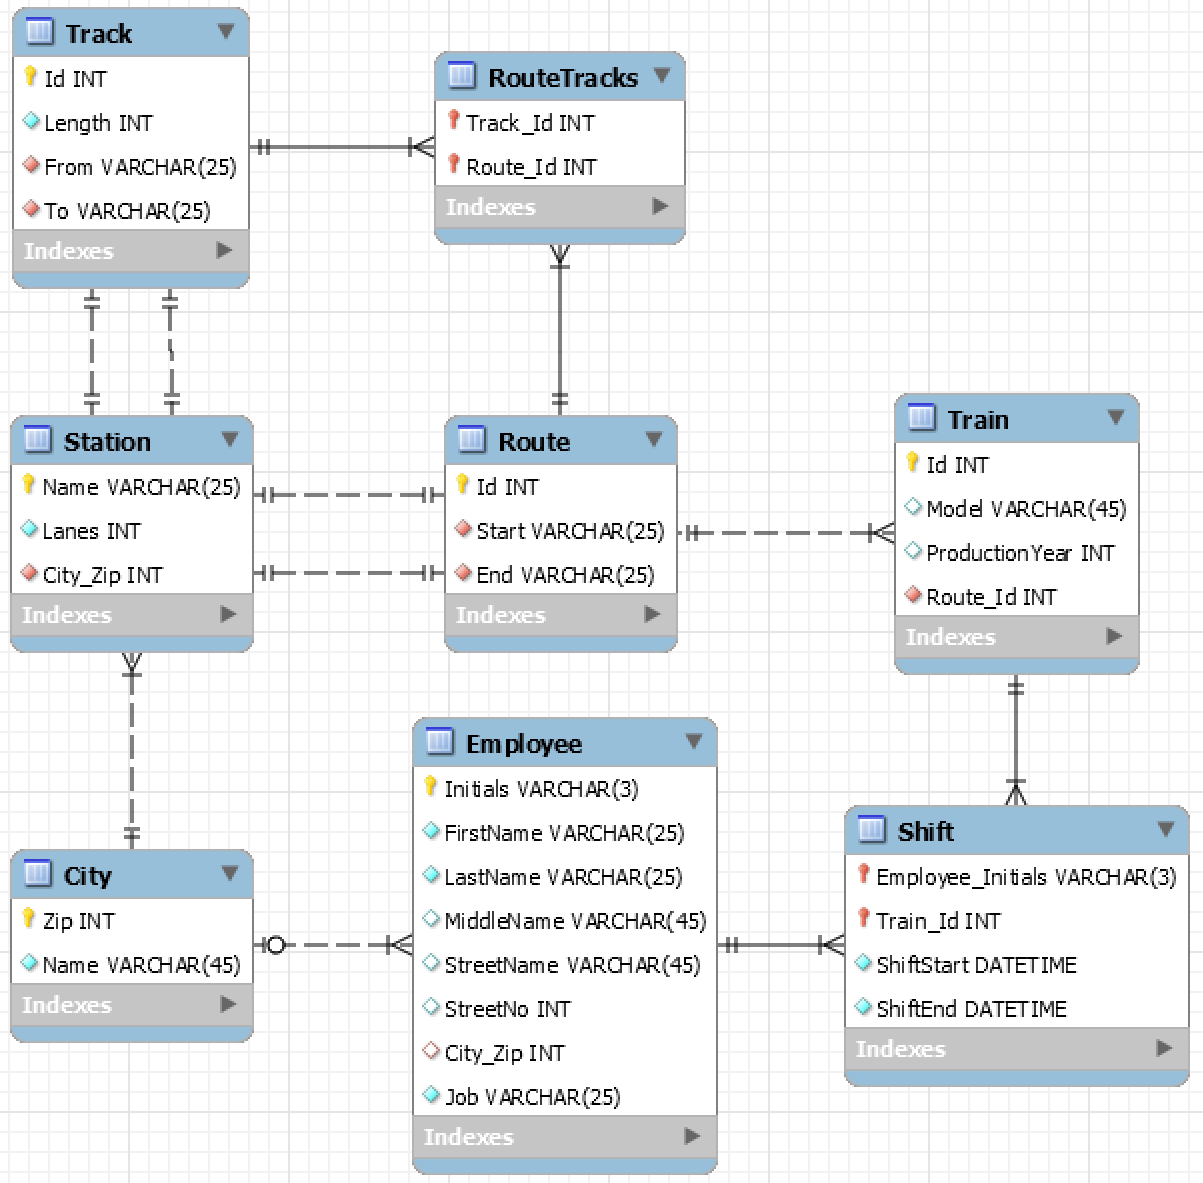
\includegraphics{img/EER.png}
    \caption{EER Diagram implemented in MySQL}
    \label{fig:EER}
\end{figure}

Although the EER diagram only is a model and not a database itself. The diagram 
representation is so precise a description of the database, that the database 
can be created from it (known as forward engineering). Likewise the databases 
can be backward engineered into diagrams, which can be a great help, when 
trying to understand an existing database. In this project forward engineering 
on the MySQL EER diagram was used to generate the SQL file shown in 
Appendix~\ref{app:db}. This single file, when run, creates the entire database 
exactly as described by the digram.


\subsection{Functionality} % Other title?

% Specs require: Functions, procedures, transactions, triggers and events
% Make sure to include all of these in the design or possibly in the intro
